\chapter{Results}
\label{cha:Results}
% \lipsum \autocite{DBLP:books/sp/HarderR01}


\section{Data Exploration}

About 45\% of the 1.8 Million prompts mention at least one artist and only 13\% of all prompts mention a style. 8\% of all prompts mention both a style and an artist, which means that 61\% of prompts with style mentions also mention at least one artist. We thus have to note, that we are in essence only using 8\% of all prompts in the dataset for the artist characterizations and subsequent dissimilarity analysis.

A total of YYY artists qualify for the artist characterization and dissimilarity analysis since they were mentioned in prompts, that included style mentions.

\begin{figure}[h]
    \begin{center}
        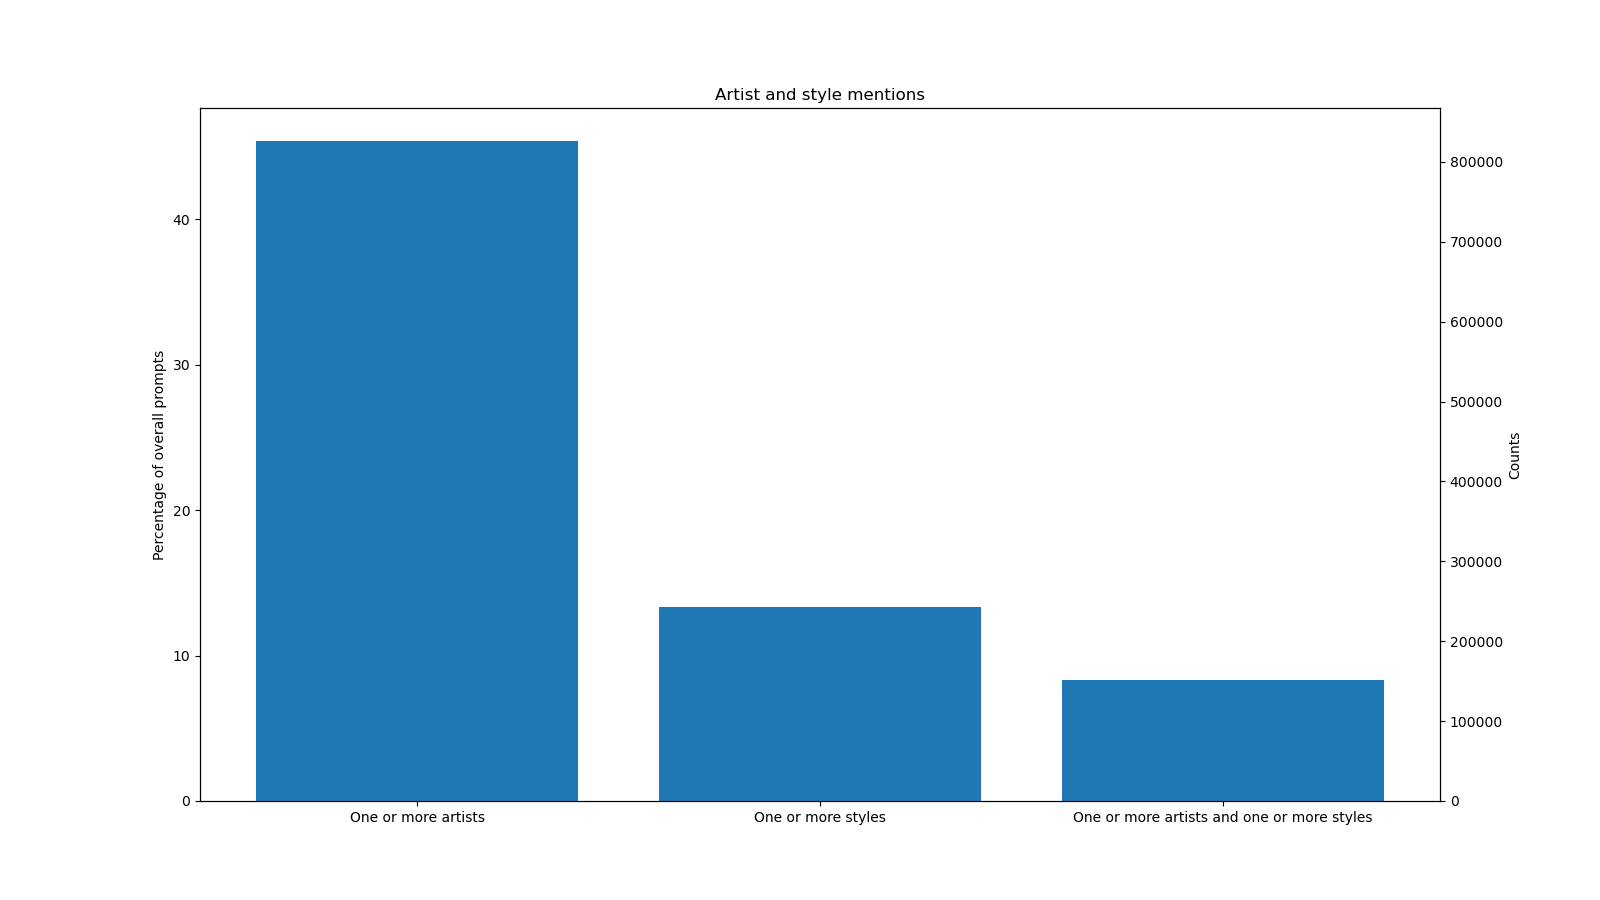
\includegraphics[height=7cm]{Bilder/artist_and_style_mentions.png}\\[2.5ex]
    \end{center}
\caption{Prompts with artist and style mentions in the dataset}
\end{figure}

\subsection{Artist Mentions}

Out of the 3477 artists from the artist dataset, 2825 were mentioned in the prompt dataset. The amount of mentions of the individual artists varies drastically, it appears to follow a Zipf distribution, similar to words in a corpus. The top 10 artists with the most mentions are shown in \ref{fig:top10_artists}, they make up a large share of the total artist mentions. The most mentioned artist 'Greg Rutkowski' appears in about 10\% of all prompts.

\begin{figure}[h]
    \begin{center}
        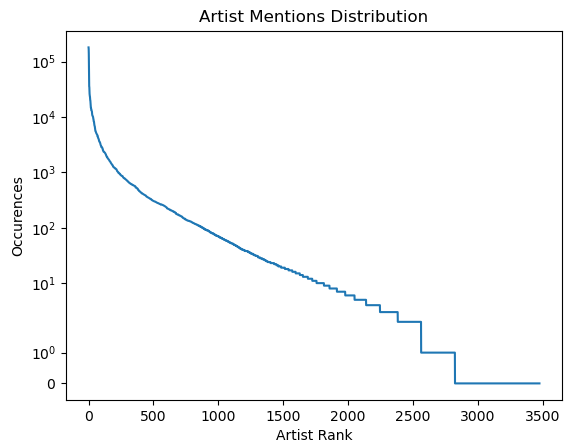
\includegraphics[height=7cm]{Bilder/artist_mentions_distribution_scale_symlog.png}\\[2.5ex]
    \end{center}
\caption{Artist mentions appear to follow a Zipf distribution}
\end{figure}

\begin{figure}[h]
    \begin{center}
        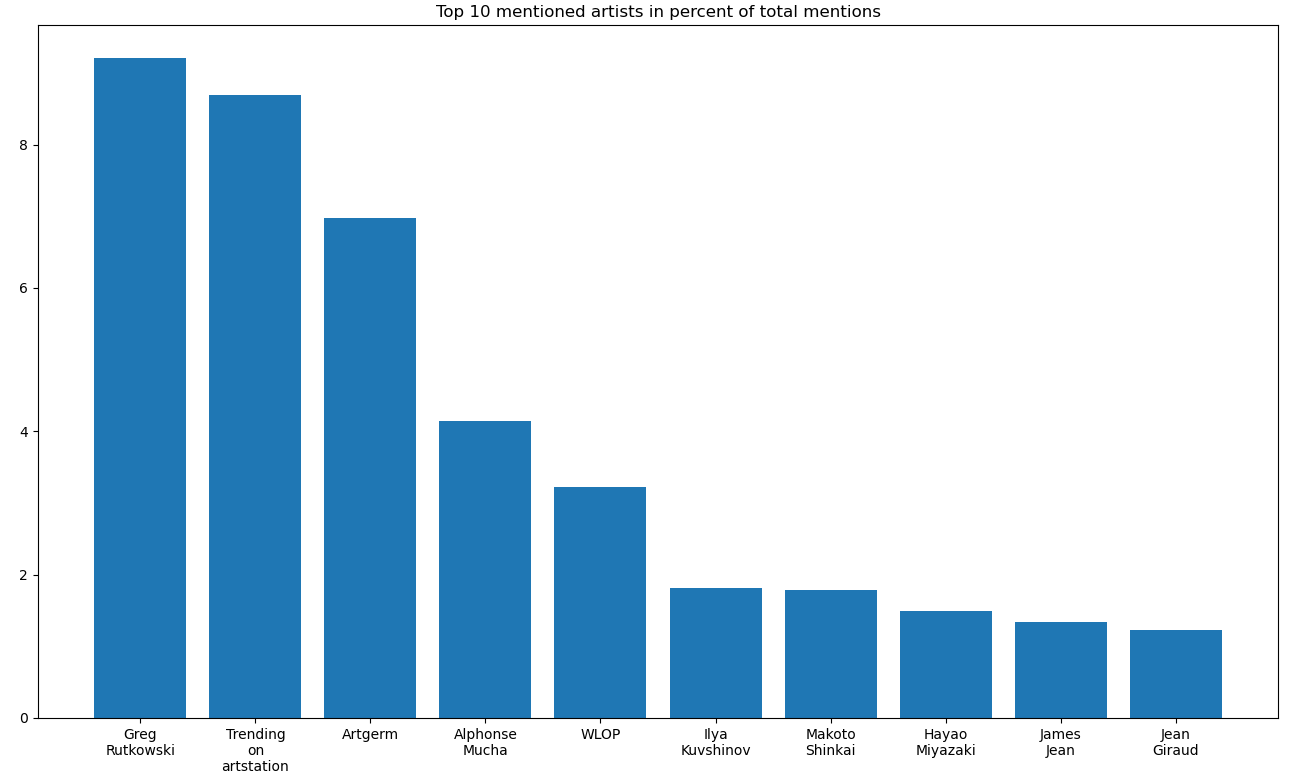
\includegraphics[height=7cm]{Bilder/top10_artists.png}\\[2.5ex]
    \end{center}
\caption{Top 10 artists with the most mentions in the dataset}
\label{fig:top10_artists}
\end{figure}


\subsection{Style Mentions}

185 of all 192 styles in the list are found in the dataset. Similarly to the artist mentions, they appear to follow a Zipf distribution.

\begin{figure}[h]
    \begin{center}
        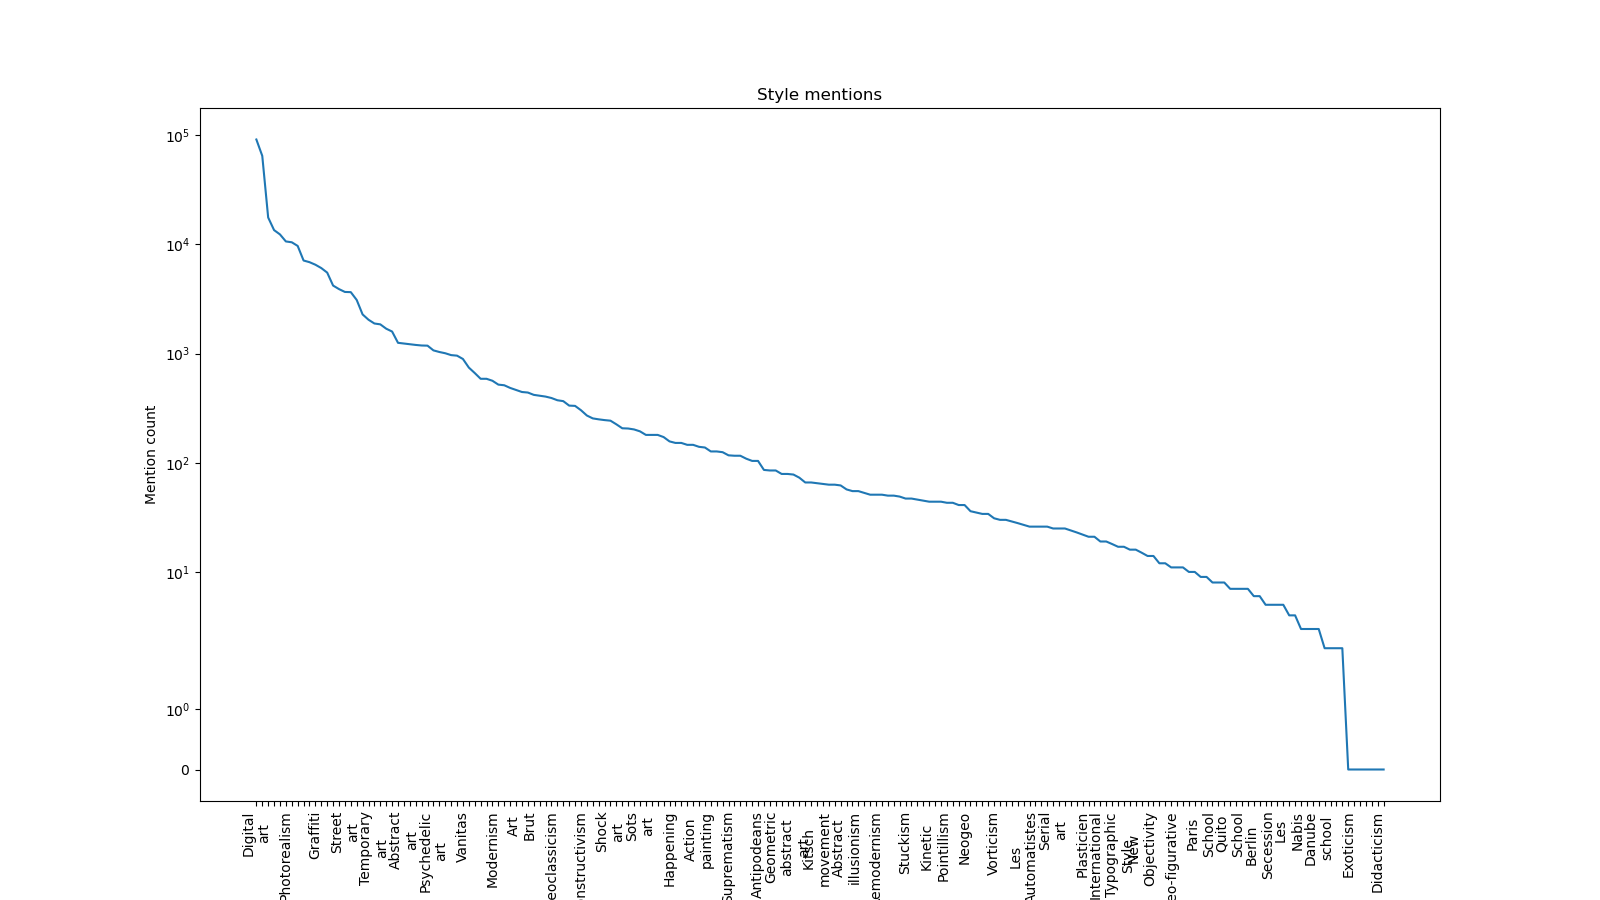
\includegraphics[height=7cm]{Bilder/styles_count_distribution_scale_symlog.png}\\[2.5ex]
    \end{center}
\caption{Style mention count distribution}
\end{figure} % style_occurences notebook

\begin{figure}[h]
    \begin{center}
        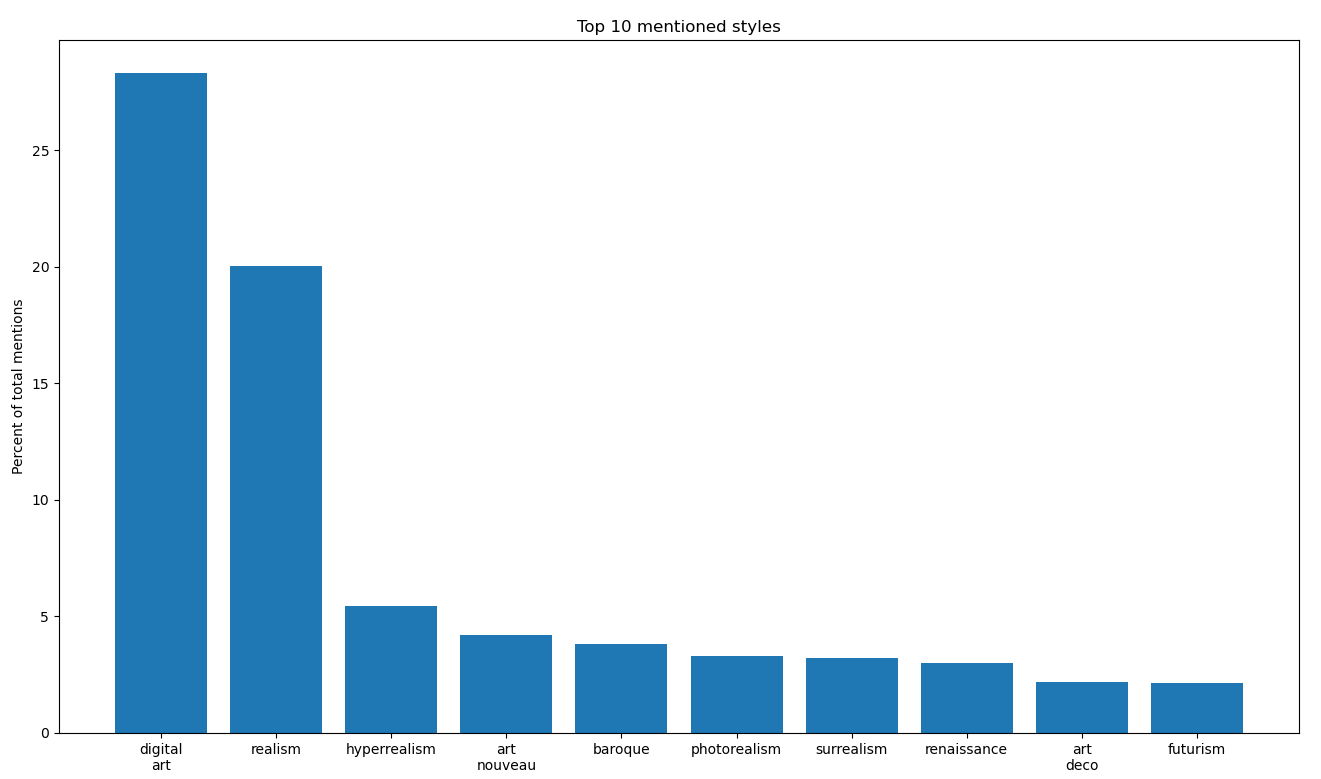
\includegraphics[height=7cm]{Bilder/top10_styles_percentages.png}\\[2.5ex]
    \end{center}
\caption{Top 10 styles with the most mentions in the dataset}
\end{figure} % style_occurences notebook

\section{Artist Characterization}

The dissimilarity computations for the artists with the highest and lowest dissimiliarity are shown below. The artist with the highest dissimiliarity is '...', this artist is only mentioned in xx prompts and only has a single style mention. Any artist with such low amounts of mentions and style mentions

\begin{figure}[h]
    \begin{center}
        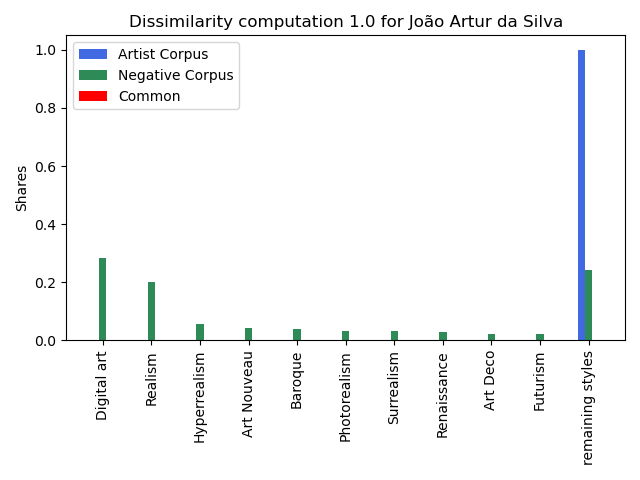
\includegraphics[height=7cm]{Bilder/artist_highest_dissimilarity.png}\\[2.5ex]
    \end{center}
\caption{Artist characterization for the artist with the highest dissimilarity}
\end{figure}

\begin{figure}[h]
    \begin{center}
        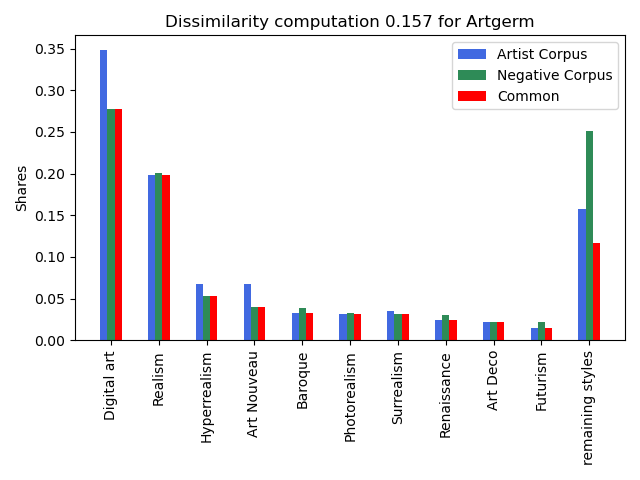
\includegraphics[height=7cm]{Bilder/artist_lowest_dissimilarity.png}\\[2.5ex]
    \end{center}
\caption{Artist characterization for the artist with the lowest dissimilarity}
\label{fig:lowest_dissimilarity}
\end{figure}


\section{Dissimilarity correlation results}

When plotting the dissimilarity values of artists sorted by their popularity, we can notice there is a relation between the rank and dissimilarity. The dissimilarity tends to increase with lower artist popularity, however this relationship does not look very strong.
The Spearman's rank correlation coefficient produces an \(r_s\) value of XXX, indicating ...
The \(p\) value of the hypothesis test is XXX, this means the Null hypothesis can be rejected with a significance level of 0.05. We can thus conclude that there is a correlation between the popularity of an artist and the dissimilarity of the artist to other artists.

TODO fix the XXX and sentence above

\begin{figure}[h]
    \begin{center}
        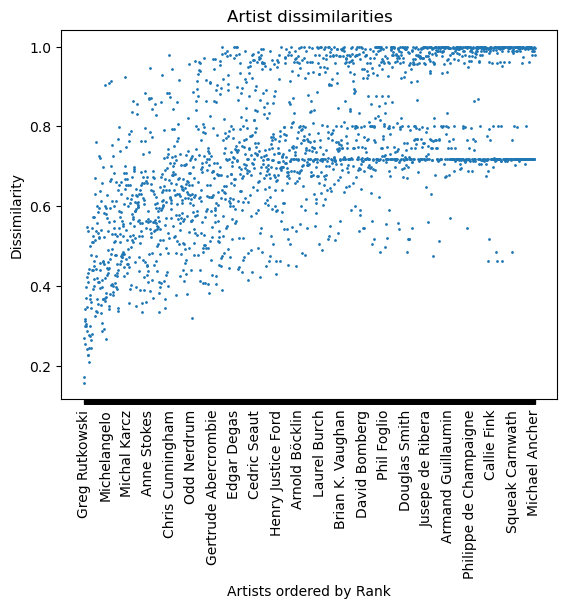
\includegraphics[height=7cm]{Bilder/ranked_artist_dissimilarity.png}\\[2.5ex]
    \end{center}
\caption{Dissimilarity values of artists sorted by their popularity}
\end{figure}


% Can we reject the null hypothesis?
% Null hypothesis: The two variables are not correlated. 
% we need a small p value to reject




TODO:

By using your method on your data, you will produce some
results (numbers, plots, etc.). Please note that any scripts
you will generate during the project should also be briefly
mentioned in the documentation. However, please do not
put source code in the documentation. Rather share with
us any scripts (and datasets) you create by means of a
repository.

TODO 15-20 Seiten

% TODO Bilder zusammenschneiden (Rand wegmachen)